\addcontentsline{toc}{chapter}{Занятие 11. Совместное распределение случайных величин}
\chapter*{Занятие 11. Совместное распределение случайных величин}

\addcontentsline{toc}{section}{Контрольные вопросы и задания}
\section*{Контрольные вопросы и задания}

\subsubsection*{Запишите основные вероятностные распределения и поясните смысл их параметров.}

Основные распределения:
\begin{enumerate}
\item дискретное распределение:
\begin{enumerate}
\item равномерное дискретное распределение
$$P \left( \xi = k \right) =
\frac{1}{N},
1 \leq k \leq N,
M \xi = \frac{N+1}{2}, D \xi = \frac{N^2 - 1}{12};$$
\item биномиальное распределение: $ \xi \sim Biom \left( n, p \right) $
$$P \left\{ \xi = k \right\} =
C_n^k p^k q^{n-k},$$
где $0 \leq k \leq n, q = 1 - p, M \xi = np, D \xi = npq$;
\item геометрическое распределение $ \xi \sim Geom \left( p \right), p \in \left( 0, 1 \right) $
$$P \left\{ \xi = k \right\} =
pq^k,
k \geq 0,
M \xi = \frac{q}{p},
D \xi = \frac{q}{p^2};$$
\item пуассоновское распределение: $ \xi \sim Pois \left( \lambda \right), \lambda > 0$
$$P \left\{ \xi = k \right\} = \frac{ \lambda^k}{k!} \cdot e^{- \lambda },
k \geq 0,
M \xi = \lambda,
D \xi = \lambda;$$
\end{enumerate}
\item непрерывные распределения:
\begin{enumerate}
\item равномерное распределение: $ \xi \sim U \left( \left[ a, b \right] \right) $
$$p \left( x \right) =
\begin{cases}
\frac{1}{b-a}, \qquad x \in \left[ a, b \right], \\
0, x \notin \left[ a, b \right], \\
\end{cases}
M \xi = \frac{a+b}{2},
D \xi = \frac{ \left( b-a \right)^2}{12};$$
\item экспоненциальное распределение: $ \xi \sim Exp \left( \lambda \right), \lambda > 0$
$$p \left( x \right) =
\begin{cases}
\lambda e^{- \lambda x}, \qquad x \geq 0, \\
0, \qquad x < 0, \\
\end{cases}
M \xi = \frac{1}{ \lambda },
D \xi = \frac{1}{ \lambda^2};$$
\item распределение Коши: $ \xi \sim C \left( \Theta \right), \Theta > 0$
$$p \left( x \right) =
\frac{ \Theta }{ \pi \left( x^2 + \Theta^2 \right) };$$
\item гауссовское (нормальное) распределение:
$$ \xi \sim \mathcal{N} \left( a, \sigma^2 \right),
a \in \mathbb{R},
\sigma^2 > 0,$$
$$p \left( x \right) = \frac{1}{ \sqrt{2 \pi } \cdot \sigma } \cdot e^{- \frac{ \left( x-a \right)^2}{2 \sigma^2}},
x \in \mathbb{R},
M \xi = a,
D \xi = \sigma^2.$$
\end{enumerate}
\end{enumerate}

\subsubsection*{Что называется случайным вектором?}

Случайный вектор --- это набор упорядоченных величин
$$ \vec{ \xi } =
\left( \xi_1, \xi_2, \dotsc, \xi_n \right).$$

\subsubsection*{Приведите критерий независимости компонент случайного вектора.}

$ \xi_1, \dotsc, \xi_n$ --- независимы тогда и только тогда, когда
$$p_{ \vec{ \xi }} \left( x_1, \dotsc, x_n \right) =
\prod \limits_{i=1}^n p_{ \xi_i} \left( x \right).$$

\subsubsection*{Как вычислить плотность суммы независимых случайных величин?}

Для независимых случайных величин
$$p_{ \xi + \eta } \left( x \right) =
\int \limits_{ \mathbb{R}} p_{ \xi } \left( x-y \right) p_{ \eta } \left(t y \right) dy.$$

\addcontentsline{toc}{section}{Аудиторные задачи}
\section*{Аудиторные задачи}

\subsubsection*{11.3}

\textit{Задание.} Пусть $ \xi, \eta $ --- независимые случайные величины, причём $ \xi $ имеет показательное распределение с параметром $ \lambda $, а $ \nu $ равномерно распределена на отрезке $ \left[ 0, h \right] $.
Найдите плотностьраспределения случайной величины $ \xi $. 

\textit{Решение.} Случайная величина $ \xi $ имеет плотность распределения
$$p_{ \xi } \left( x \right) =
\begin{cases}
\lambda e^{- \lambda x}, \qquad x \geq 0, \\
0, \qquad x < 0.
\end{cases}$$

Случайная величина $ \eta $ имеет плотность распределения
$$p_{ \eta } \left( x \right) =
\begin{cases}
0, \qquad x \notin \left[ 0, h \right], \\
\frac{1}{h}, \qquad x \in \left[ 0, h \right].
\end{cases}$$

Случайные величины $ \xi, \eta $ --- независимы.
Записываем плотность распределения суммы
$$p_{ \xi + \eta } \left( x \right) =
\int \limits_{ \mathbb{R}} p_{ \xi } \left( x - y \right) p_{ \eta } \left( y \right) dy.$$
Будем использовать индикатор
$$p_{ \xi + \eta } \left( x \right) =
\int \limits_{ \mathbb{R}} \lambda e^{- \lambda \left( x-y \right) } \cdot
\mathbbm{1} \left( x-y \geq 0 \right) \cdot
\frac{1}{h} \cdot
\mathbbm{1} \left( y \in \left[ 0, h \right] \right) dy.$$
Эти индикаторы будут задавать, где именно будем интегрировать эти плотности.
Должны интегрировать по пересечению $ \left[ 0, h \right] \cap \left( - \infty, x \right)$, где $h$ --- фиксированное число, а $x$ --- параметр
$$p_{ \xi + \eta } \left( x \right) =
\begin{cases}
0, \qquad x < 0, \\
\int \limits_0^x \lambda e^{- \lambda \left( x-y \right) } dy \cdot \frac{1}{h}, \qquad x \in \left[ 0, h \right], \\
\int \limits_0^h \lambda e^{- \lambda \left( x-y \right) } dy \cdot \frac{1}{h}, \qquad x > h.
\end{cases}$$

Отдельно вычисляем каждый интеграл.
Второй случай
$$ \frac{ \lambda }{h} \int \limits_0^x e^{- \lambda x} \cdot e^{ \lambda y} dy =
\left. \frac{1}{h} \cdot e^{- \lambda x} \cdot e^{ \lambda y} \right|_0^x =
\frac{1}{h} \cdot e^{- \lambda x} \cdot e^{ \lambda x} - \frac{1}{h} \cdot e^{- \lambda x} \cdot e^0.$$
Выражение $e^{- \lambda x} \cdot e^{ \lambda x}$ даёт единицу
$$\frac{ \lambda }{h} \int \limits_0^x e^{- \lambda x} \cdot e^{ \lambda y} dy =
\frac{1}{h} - \frac{1}{h} \cdot e^{- \lambda x} =
\frac{1}{h} \left( 1 - e^{- \lambda x} \right) =
\frac{1-e^{- \lambda x}}{h}.$$

Вычисляем третий случай --- такой же итеграл, только в пределах от нуля до $h$.
Имеем
$$ \int \limits_0^h \lambda e^{- \lambda \left( x-y \right) } dy \cdot \frac{1}{h} =
\left. \frac{1}{h} \cdot e^{- \lambda x} \cdot e^{ \lambda y} \right|_0^h =
\frac{e^{- \lambda x}}{h} \left( e^{ \lambda h} - 1 \right),$$
где $x$ --- это параметр.
Следовательно
$$p_{ \xi + \eta } \left( x \right) =
\begin{cases}
0, \qquad x < 0, \\
\frac{1-e^{- \lambda x}}{h}, \qquad x \in \left[ 0, h \right], \\
\frac{e^{- \lambda x}}{h} \left( e^{ \lambda h} - 1 \right), \qquad x > h.
\end{cases}$$

\subsubsection*{11.4}

\textit{Задание.} Пусть $ \xi, \eta, \zeta $ --- независимые случайные величины.
Известно,
что $ \xi $ и $ \eta $ имеют функции распределения $F$ и $G$ соответственно,
а $ \zeta $ принимат значения 0 или 1 с вероятностями $p$ и $q$ соответственно $ \left( p + q = 1 \right) $.
Найдите функцию распределения случайной величины $ \zeta \xi + \left( 1 - \zeta \right) \eta $.

\textit{Решение.} Начинаем с определения функции распределения
$$P \left( \xi \leq x \right) = F_{ \xi } \left( x \right) = F,
P \left( \eta \leq x \right) = G.$$

По условию $P \left( \zeta = 0 \right) = p = 1 - P \left( \zeta = 1 \right) = 1 - q$.

Откуда $P \left( \zeta = 1 \right) = q$.

Ищем функцию распределения по определению
$$F_{ \zeta \xi + \left( 1 - \zeta \right) \eta } \left( x \right) =
P \left(  \zeta \xi + \left( 1 - \zeta \right) \eta \leq x \right).$$
Применяем формулу полной вероятности.
Если $ \zeta = 0$, то случайная величина --- это $ \eta $, если $ \zeta = 1$, то это $ \xi $.
Получаем
$$F_{ \zeta \xi + \left( 1 - \zeta \right) \eta } \left( x \right) =
P \left( \zeta = 0 \right) P \left( \eta \leq x \right) + P \left( \zeta = 1 \right) P \left( \eta \leq x \right) =
pG + \left( 1 - p \right) F.$$
В итоге получаем $F_{ \zeta \xi + \left( 1 - \zeta \right) \eta } \left( x \right) = pG + qF.$

\subsubsection*{11.5}

\textit{Задание.} Пусть $ \xi $ --- случайная величина с функцией распределения $F$.
Найдите функцию распределения случайного вектора $ \left( \xi, \left| \xi \right| \right) $.

\textit{Решение.} Есть случайный вектор, который имеет две компоненты.
Поэтому функция распределения будет иметь 2 аргумента.

По определению $F_{ \left( \xi, \left| \xi \right| \right) } \left( x, y \right) = P \left( \xi \leq x, \left| \xi \right| \leq y \right).$
Раскрываем модуль $F_{ \left( \xi, \left| \xi \right| \right) } \left( x, y \right) = P \left( \xi \leq x, -y \leq \xi \leq y \right) $.
Всё касается одной и той же случайной величины
$$F_{ \left( \xi, \left| \xi \right| \right) } \left( x, y \right) =
\begin{cases}
0, \qquad x < - y, \\
P \left( \xi \in \left[ -y, x \right] \right), \qquad x \in \left[ -y, y \right], \\
P \left( \xi \in \left[ -y, y \right] \right), \qquad x > y
\end{cases}
\cdot \mathbbm{1} \left( y > 0 \right).$$
Выражаем это через функцию распределения $ \xi $.
Получаем
$$F_{ \left( \xi, \left| \xi \right| \right) } \left( x, y \right) =
\begin{cases}
0, \qquad x < - y, \\
F_{ \xi } \left( x \right) - F_{ \xi } \left( -y \right), \qquad x \in \left[ -y, y \right], \\
F_{ \xi } \left( y \right) - F_{ \xi } \left( -y \right), \qquad x > y
\end{cases}
\cdot \mathbbm{1} \left( y > 0 \right).$$

\subsubsection*{11.6}

\textit{Задание.}
Случайный вектор $ \left( \xi_1, \xi_2 \right) $ имеет плотность распределения
$$p \left( x \right) =
\left( x+ay^2 \right) \cdot \mathbbm{1}_{ \left[ 0, 1 \right]^2}.$$
Найдите:
\begin{enumerate}[label=\alph*)]
\item параметр $a$;
\item $M \xi_1, M \xi_1 \xi_2, P \left( \xi_1 < \xi_2 \right) $;
\item плотности $p_{ \xi_1} \left( x \right), p_{ \xi_2} \left( x \right) $;
\item плотность распределения случайной величины $ \max \left( \xi_1, \xi_2 \right) $.
\end{enumerate}
Являются ли $ \xi_1, \xi_2$ независимыми?

\textit{Решение.}
\begin{enumerate}[label=\alph*)]
\item Находим неизвестный параметр $a$, который входит в плотность из условия нормировки.

Плотность определена, когда $0 \leq x \leq 1, 0 \leq y \leq 1$.

Условие нормировки выполняется для всякой плотности
$$1 =
\int \limits_{- \infty }^{+ \infty } \int \limits_{- \infty }^{+ \infty } p \left( x, y \right) dxdy =
\int \limits_0^1 \int \limits_0^1 \left( x+ay^2 \right) dxdy.$$
Подставляем пределы интегрирования
$$1 =
\left. \int \limits_0^1 \left( \frac{x^2}{2} + ay^2 x \right) \right|_0^1 dy =
\int \limits_0^1 \left( \frac{1}{2} + ay^2 \right) dy =
\frac{1}{2} + \frac{a}{3}.$$
Отсюда следует, что
$$a =
\frac{2}{3};$$
\item ищем $M \xi_1$.
Математическое ожидание $ \phi \left( \xi_1, \xi_2 \right) $ вычислили бы так
$$M \phi \left( \xi_1, \xi_2 \right) =
\iint_{ \mathbb{R}^2} \phi \left( x, y \right) p \left( x, y \right) dxdy,$$
где $p$ --- это их совместная вероятность, то есть вероятность вектора.

В данном случае $ \phi \left( \xi_1, \xi_2 \right) = \xi_1$.

Вычисляем математическое ожидание
$$M \xi_1 =
\iint_{ \mathbb{R}^2} x \cdot p \left( x, y \right) dxdy =
\int \limits_0^1 \int \limits_0^1 x \left( x + ay^2 \right) dxdy.$$
Раскрываем скобки
$$M \xi_1 =
\int \limits_0^1 \int \limits_0^1 \left( x^2 + ay^2 x \right) dxdy =
\left. \int \limits_0^1 \left( \frac{x^3}{3} + \frac{ay^2 x^2}{2} \right) \right|_0^1 dy.$$
Подставляем пределы интегрирования
$$M \xi_1 =
\int \limits_0^1 \left( \frac{1}{3} + \frac{ay^2}{2} \right) dy =
\left. \left( \frac{y}{3} + \frac{ay^3}{6} \right) \right|_0^1 =
\frac{1}{3} + \frac{a}{6}.$$
Подставляем
$$a =
\frac{2}{3}.$$
Получаем
$$M \xi_1 =
\frac{1}{3} + \frac{3}{2 \cdot 6} =
\frac{1}{3} + \frac{1}{4}.$$
Приводим к общему знаменателю, для чего первое слагаемое умножаем и делим на 4, а второе --- на 3
$$M \xi_1 =
\frac{7}{12}.$$

Найдём следующее математическое ожидание.

В данном случае $ \phi \left( \xi_1, \xi_2 \right) = \xi_1 \xi_2$.

Это будет
$$M \xi_1 \xi_2 =
\iint_{ \mathbb{R}^2} xyp \left( x, y \right) dxdy.$$
Подставляем вид $p \left( x, y \right) $.
Получаем
$$M \xi_1 \xi_2 =
\int \limits_0^1 \int \limits_0^1 xy \left( x + \frac{3}{2} \cdot y^2 \right) dxdy =
\int \limits_0^1 \int \limits_0^1 \left( x^2 y + \frac{3xy^3}{2} \right) dxdy.$$
Берём внутненний интеграл
$$M \xi_1 \xi_2 =
\int \limits_0^1 \left( \frac{y}{3} + \frac{3y^3}{4} \right) dy =
\left. \left( \frac{y^2}{6} + \frac{3y^4}{16} \right) \right|_0^1 =
\frac{1}{6} + \frac{3}{16} =
\frac{17}{48}.$$

Любую вероятность можно записать как математическое ожидание индикатора
$$P \left( \xi_1 < \xi_2 \right) =
M \mathbbm{1} \left( \xi_1 < \xi_2 \right).$$
В данный момент $\mathbbm{1} \left( \xi_1 < \xi_2 \right) = \phi \left( \xi_1, \xi_2 \right) $.
Поэтому
$$P \left( \xi_1 < \xi_2 \right) =
\iint_{ \mathbb{R}^2} \mathbbm{1} \left( x < y \right) p \left( x, y \right) dxdy =
\iint_{x < y} p \left( x, y \right) dxdy.$$
Подставляем плотность распределения
$$P \left( \xi_1 < \xi_2 \right) =
\int \limits_0^1 \int \limits_0^y \left( x + \frac{3y^2}{2} \right) dxdy =
\left. \int \limits_0^1 \left( \frac{x^2}{2} + \frac{2y^2 x}{2} \right) \right|_0^y.$$
Подставляем пределы интегрирования
$$P \left( \xi_1 < \xi_2 \right) =
\int \limits_0^1 \left( \frac{y^2}{2} + \frac{3y^3}{2} \right) dxdy =
\left. \left( \frac{y^3}{6} + \frac{3y^4}{8} \right) \right|_0^1 =
\frac{1}{6} + \frac{3}{8}.$$
Приводим к общему знаменателю.
Для этого первую дробь умножаем и делим на 4, а вторую --- на 3
$$P \left( \xi_1 < \xi_2 \right) =
\frac{4+9}{24} =
\frac{13}{24};$$
\item находим плотность каждой из случайных величин.
Находим как плотности компонент вектора
$$p_{ \xi_1} \left( x \right) =
\int \limits_{ \mathbb{R}} p \left( x, y \right) dy =
\int \limits_0^1 \left( x + \frac{3y^2}{2} \right) dy \cdot \mathbbm{1} \left( x \in \left[ 0, 1 \right] \right).$$
Вычисляем интеграл
$$p_{ \xi_1} \left( x \right) =
\left. \left( xy + \frac{3y^3}{6} \right) \right|_0^1 \cdot \mathbbm{1} \left( x \in \left[ 0, 1 \right] \right) =
\left. \left( xy + \frac{y^3}{2} \right) \right|_0^1 \cdot \mathbbm{1} \left( x \in \left[ 0, 1 \right] \right).$$
Подставляем пределы интегрирования
$$p_{ \xi_1} \left( x \right) =
\left( x + \frac{1}{2} \right) \cdot \mathbbm{1} \left( x \int \left[ 0, 1 \right] \right).$$

Теперь ищем плотность $ \xi_2$ аналогичным образом
$$p_{ \xi_2} \left( y \right) =
\int \limits_{ \mathbb{R}} p \left( x, y \right) dx =
\int \limits_0^1 \left( x + \frac{3y^2}{2} \right) dx \cdot \mathbbm{1} \left( y \in \left[ 0, 1 \right] \right).$$
Вычисляем интеграл
$$p_{ \xi_2} \left( y \right) =
\left. \left( \frac{x^2}{2} + \frac{3y^2 x}{2} \right) \right|_0^1 \cdot \mathbbm{1} \left( y \in \left[ 0, 1 \right] \right) =
\left( \frac{1}{2} + \frac{2y^2}{2} \right) \cdot \mathbbm{1} \left( y \in \left[ 0, 1 \right] \right).$$

Поскольку совместная плотность $p_{ \vec{ \xi }} \left( x, y \right) \neq p_{ \xi_1} \left( x \right) \cdot p_{ \xi_2} \left( y \right) $,
то $ \xi_1$ и $ \xi_2$ не могут быть независимыми;
\item $F_{ \max \left( \xi_1, \xi_2 \right) } \left( x \right) $ --- ищем.

$$P \left( \max \left( \xi_1, \xi_2 \right) \leq x \right) =
P \left( \xi_1 \leq x, \xi_2 \leq x \right) =
M \mathbbm{1} \left( \xi_1 \leq x, \xi_2 \leq x \right).$$
Вычисляем математическое ожидание по определению
$$P \left( \max \left( \xi_1, \xi_2 \right) \leq x \right) =
\iint_{ \mathbb{R}^2} \mathbbm{1} \left( u \leq x, v \leq x \right) \cdot p \left( u, v \right) dudv.$$
При этом $x \in \left[ 0, 1 \right] $.
Получаем
$$P \left( \max \left( \xi_1, \xi_2 \right) \leq x \right) =
\int \limits_0^x \int \limits_0^x \left( u + \frac{3v^2}{2} \right) dudv =
\left. \int \limits_0^x \left( \frac{u^2}{2} + \frac{3u^2 \cdot u}{2} \right) \right|_0^x dv.$$
Подставляем пределы интегрирования
$$P \left( \max \left( \xi_1, \xi_2 \right) \leq x \right) =
\int \limits_0^x \left( \frac{x^2}{2} + \frac{3v^2 x}{2} \right) dv =
\frac{x^3}{2} + \frac{x^4}{2}, x \in \left[ 0, 1 \right].$$

Записываем функцию распределения
$$F_{ \max \left( \xi_1, \xi_2 \right) } \left( x \right) =
\begin{cases}
0, \qquad x < 0, \\
\frac{x^3}{2} + \frac{x^4}{2}, \qquad x \in \left[ 0, 1 \right], \\
1, \qquad x > 1.
\end{cases}$$

Ищем плотность распределения
$$p_{ \max \left( \xi_1, \xi_2 \right) } \left( x \right) =
F_{ \max \left( \xi_1, \xi_2 \right) }' \left( x \right) =
\left( \frac{3}{2} \cdot x^2 + 2x^3 \right) \cdot \mathbbm{1} \left( x \in \left[ 0, 1 \right] \right).$$
\end{enumerate}

\subsubsection*{11.7}

\textit{Задание.} Пусть $ \xi_1, \xi_2$ --- независимые случайные величины со стандартным нормальным распределением каждая.
Найдите плотность оаспределения случайной величины $ \sqrt{ \xi_1^2 + \xi_2^2}$.

\textit{Решение.} Выпишем плотность $ \xi_1, \xi_2$ каждую из условия, $ \sigma = 1, a = 0$.
Имеем
$$p_{ \xi_1} \left( x \right) =
p_{ \xi_2} \left( x \right) =
\frac{1}{ \sqrt{2 \pi }} \cdot e^{- \frac{x^2}{2}}.$$

Тогда совместная плотность вектора (из независимости)
$$p_{ \left( \xi_1, \xi_2 \right) } \left( x, y \right) =
p_{ \xi_1} \left( x \right) \cdot p_{ \xi_2} \left( x \right) =
\frac{1}{2 \pi } \cdot e^{- \frac{x^2 + y^2}{2}}.$$

Функция распределения этой случайной величины по определению
$$F_{ \sqrt{ \xi_1^2 + \xi_2^2}} \left( t \right) =
P \left( \sqrt{ \xi_1^2 + \xi_2^2} \leq t \right).$$
Это целесообразно рассматривать при $t \geq 0$.
Записываем вероятность как индикатор этого события $F_{ \sqrt{ \xi_1^2 + \xi_2^2}} \left( t \right) = M \mathbbm{1} \left( \sqrt{ \xi_1^2 + \xi_2^2} \leq t \right) $.
Есть две случайные величины, значит будет двойной интеграл
$$F_{ \sqrt{ \xi_1^2 + \xi_2^2}} \left( t \right) =
\iint_{ \mathbb{R}^2} \mathbbm{1} \left( \sqrt{x^2 + y^2} \leq t \right) p_{ \left( \xi_1, \xi_2 \right) } \left( x, y \right) dxdy.$$
Перепишем плотность
$$F_{ \sqrt{ \xi_1^2 + \xi_2^2}} \left( t \right) =
\iint_{ \mathbb{R}^2} \mathbbm{1} \left( \sqrt{x^2 + y^2} \leq t \right) \cdot \frac{1}{2 \pi } \cdot e^{- \frac{x^2 + y^2}{2}} \cdot dxdy.$$
Перейдём в полярную систему координат
$x = \rho \cos \phi,
y = \rho \sin \phi,
dxdy = \\
= \rho d \rho d \phi,
\rho: 0 \rightarrow t,
\phi: 0 \rightarrow 2 \pi,
x^2 + y^2 = \rho^2,
\mathbbm{1} \left( \sqrt{x^2 + y^2} \leq t \right) = \mathbbm{1} \left( \rho \leq t \right) $.
Получаем
$$F_{ \sqrt{ \xi_1^2 + \xi_2^2}} \left( t \right) =
\int \limits_0^{2 \pi } \int \limits_0^t \frac{1}{2 \pi } \cdot e^{- \frac{ \rho^2}{2}} \rho d \rho d \phi.$$
По $d \phi $ проинтегрируем сразу
$$F_{ \sqrt{ \xi_1^2 + \xi_2^2}} \left( t \right) =
- \int \limits_0^t d \left( e^{- \frac{ \rho^2}{2}} \right) =
\left. - e^{- \frac{ \rho^2}{2}} \right|_0^t =
1 - e^{- \frac{t^2}{2}}$$
--- это при $t > 0$.

Нужно продифференцировать по $t$.
Получаем
$$p_{ \sqrt{ \xi_1^2 + \xi_2^2}} \left( t \right) =
- e^{- \frac{t^2}{2}} \cdot \left( - \frac{2t}{2} \right) \cdot \mathbbm{1} \left( t > 0 \right) =
te^{- \frac{t^2}{2}} \cdot \mathbbm{1} \left( t > 0 \right).$$

\addcontentsline{toc}{section}{Домашнее задание}
\section*{Домашнее задание}

\subsubsection*{11.13}

\textit{Задание.} Пусть $ \xi $ и $ \eta $ --- независимые одинаково распределённые случайные величины с плотностью распределения
$$p \left( x \right) =
\frac{e{- \left| x \right| }}{2}.$$
Найдите плотность распределения суммы $ \xi + \eta $.

\textit{Решение.} Записываем по определению
$$p_{ \xi + \eta } \left( x \right) =
\int \limits_{ \mathbb{R}} p \left( x-y \right) p \left( y \right) dy =
\int \limits_{ \mathbb{R}} \frac{e^{- \left| x-y \right| }}{2} \cdot \frac{e^{- \left| y \right| }}{2} dy.$$
Выносим константы за знак интеграла
$$p_{ \xi + \eta } \left( x \right) =
\frac{1}{4} \int \limits_{ \mathbb{R}} e^{- \left| x-y \right| - \left| y \right| } dy =
\frac{1}{4} \cdot I.$$

Рассматриваем три случая: $x < 0, x = 0$ и $x > 0$.
В первом случае
$$I =
\int \limits_{- \infty }^x e^{-x+y+y} dy + \int \limits_x^0 e^{x-y+y} dy + \int_0^{+ \infty } e^{x-y-y} dy.$$
Во втором слагаемом $y$ уничтожается
$$I =
\int \limits_{- \infty }^x e^{2y-x} dy + \int \limits_x^0 e^x dy + \int \limits_0^{+ \infty } e^{-2y+x} dy.$$
Вычисляем интегралы
$$I =
\left. \frac{1}{2} \cdot e^{2y-x} \right|_{- \infty }^x + \left. e^x \cdot y \right|_x^0 - \left. \frac{1}{2} \cdot e^{-2y+x} \right|_0^{+ \infty }.$$
Подставляем пределы интегрирования
$$I =
\frac{1}{2} \cdot e^{2 \cdot x - x} - \frac{1}{2} \cdot e^{- \infty } + e^x \cdot 0 - e^x \cdot x - \frac{1}{2} \cdot e^{- \infty } + \frac{1}{2} \cdot e^x.$$
Экспонента на $- \infty $ равна нулю
$$I =
\frac{1}{2} \cdot e^x - x \cdot e^x + \frac{1}{2} \cdot e^x =
e^x - x \cdot e^x =
e^x \left( 1 - x \right).$$

При $x = 0$ получаем
$$I =
\int_{- \infty }^{+ \infty } e^{- \left| -y \right| - \left| y \right| } dy =
\int \limits_{- \infty }^0 e^{- \left( -y \right) + y} dy + \int \limits_0^{+ \infty } e^{-y-y} dy.$$
Упрощаем степени в экспонентах
$$I =
\int \limits_{- \infty }^0 e^{2y} dy + \int \limits_0^{+ \infty } e^{-2y} dy =
\left. \frac{1}{2} \cdot e^{2y} \right|_{- \infty }^0 - \left. \frac{1}{2} \cdot e^{-2y} \right|_0^{+ \infty }.$$
Подставляем пределы интегрирования
$$I =
\frac{1}{2} \cdot e^0 - \frac{1}{2} \cdot e^{- \infty } - \frac{1}{2} \cdot e^{- \infty } + \frac{1}{2} \cdot e^0.$$
Экспонента на $- \infty $ равна нулю
$$I =
\frac{1}{2} + \frac{1}{2} =
1.$$

В третьем случае
$$I =
\int \limits_{- \infty }^0 e^{-x+y+y} dy + \int \limits_0^x e^{-x+y-y} dy + \int \limits_x^{+ \infty } e^{x-y-y} dy.$$
Во втором слагаемом $y$ уничтожается
$$I =
\int \limits_{- \infty }^0 e^{2y-x} dy + \int \limits_0^x e^{-x} dy + \int \limits_x^{+ \infty } e^{-2y+x} dy.$$
Вычисляем интегралы
$$I =
\frac{1}{2} \cdot e^{-x} - \frac{1}{2} \cdot e^{- \infty } + e^{-x} \cdot x - e^{-x} \cdot 0 - \frac1{1}{2} \cdot e^{- \infty } + \frac{1}{2} \cdot e^{-2x+x}.$$
Экспонента на $- \infty $ равна нулю
$$I =
\frac{1}{2} \cdot e^{-x} + x \cdot e^{-x} + \frac{1}{2} \cdot e^{-x} =
e^{-x} + x \cdot e^{-x} =
e^{-x} \left( 1+x \right).$$

В итоге получаем
$$p_{ \xi + \eta } \left( x \right) =
\begin{cases}
\frac{1}{4} \cdot e^{ \left| x \right| } \left( 1 + \left| x \right| \right), \qquad x \neq 0, \\
\frac{1}{4}, \qquad x = 0.
\end{cases}$$

\subsubsection*{11.14}

\textit{Задание.}
Пусть $ \xi $ и $ \eta $ --- независимые случайные величины,
причём $ \xi $ имеет равномерное распределение на отрезке $ \left[ 0, 1 \right] $,
а $ \eta $ принимает значения $0, \pm 1, \pm 2, \dotsc $ с вероятностями $p_0, p_1, p_{-1}, \dotsc $ соответственно:
$$p_0 + p_1 + p_{-1} + \dotsc =
1.$$
Найдите плотность распределения суммы $ \xi + \eta $.

\textit{Решение.} Найдём функцию распределения суммы случайных величин по определению и применим формулу полной вероятности
$$F_{ \xi + \eta } \left( x \right) =
P \left( \xi + \eta \leq x \right) =
\sum \limits_{k = - \infty }^{+ \infty } P \left( \left. \xi + \eta \leq x \right| \eta = k \right) \cdot P \left( \eta = k \right).$$
Подставим $ \eta = k$ в условной вероятности и значение вероятности из условия.
А так же заменим вероятность на функцию распределения
$$F_{ \xi + \eta } \left( x \right) =
\sum \limits_{k = - \infty }^{+ \infty } P \left( \eta = k \right) \cdot P \left( \xi + k \leq x \right) =
\sum \limits_{k = - \infty }^{+ \infty } p_k \cdot F_{ \xi } \left( x-k \right).$$

Найдём плотность распределения как производную от функции распределения и запишем плотность распределения из условия
$$p_{ \xi + \eta } \left( x \right) =
\sum \limits_{k = - \infty }^{+ \infty } p_k \cdot p_{ \xi } \left( x-k \right) =
\sum \limits_{k = - \infty }^{+ \infty } p_k \cdot \mathbbm{1} \left( x-k \in \left[ 0, 1 \right] \right).$$
Перенесём $x$ вправо и умножим на $-1$ левую и правую части
$$p_{ \xi + \eta } \left( x \right) =
\sum \limits_{k = - \infty }^{+ \infty } p_k \cdot \mathbbm{1} \left( -k \in \left[ -x, 1-x \right] \right) =
\sum \limits_{k = - \infty }^{+ \infty } p_k \cdot \mathbbm{1} \left( k \in \left[ x-1, x \right] \right).$$
Изменим пределы интегрирования за счёт индикатора и запишем сумму в явном виде
$$p_{ \xi + \eta } \left( x \right) =
\sum \limits_{k =x-1}^{x} p_k =
p_{x-1} + p_x.$$

\subsubsection*{11.15}

\textit{Задание.} Пусть $ \xi $ --- случайная величина с функцией распределения $F$.
Найдите функцию распределения случайного вектора $ \left) \xi, \xi \right) $.

\textit{Решение.} Есть случайный вектор, который имеет две компоненты.
Поэтому фукция распределения будет иметь 2 аргумента.

По определению $F_{ \left( \xi, \xi \right) } \left( x, y \right) = P \left( \xi \leq x, \xi \leq y \right) $.
Всё касается одной и той же случайной величины.
Изображаем все случаи на рисунке $ \ref{fig:1115}$.

\begin{figure}[h!]
  \centering
  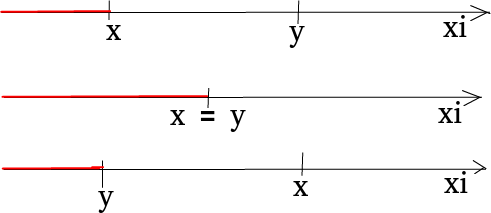
\includegraphics[width=.8\textwidth]{./pictures/11_15.png}
  \caption{Возможные случаи}
  \label{fig:1115}
\end{figure}

Получаем
$$F_{ \left( \xi, \xi \right) } \left( x, y \right) =
\begin{cases}
P \left( \xi \leq x \right), \qquad x \leq y, \\
P \left( \xi \leq y \right), \qquad x > y.
\end{cases}$$

Выражаем это через функцию распределения
$$F_{ \left( \xi, \xi \right) } \left( x, y \right) =
\begin{cases}
F \left( x \right), \qquad x \leq y, \\
F \left( y \right), \qquad x > y.
\end{cases} =
F \left( \min \left( x, y \right) \right).$$
